\section{Analysis} 

\subsection{Key information}

\subsubsection*{Images}
\begin{figure}[H]
    \centering
    \includegraphics[width=1\textwidth]{images/teachingAboutNature.png}
    \caption{Snapshot of an active classroom, demonstrating alignment towards youth, teaching, knowledge and life under water}
    \label{fig:teach}
\end{figure}  

\begin{figure}[H]
    \centering
    \includegraphics[width=1\textwidth]{images/ProNature.png}
    \caption{Snapshot of environment, demonstrating alignment towards life on land}
    \label{fig:nature}
\end{figure}  

\begin{figure}[H]
    \centering
    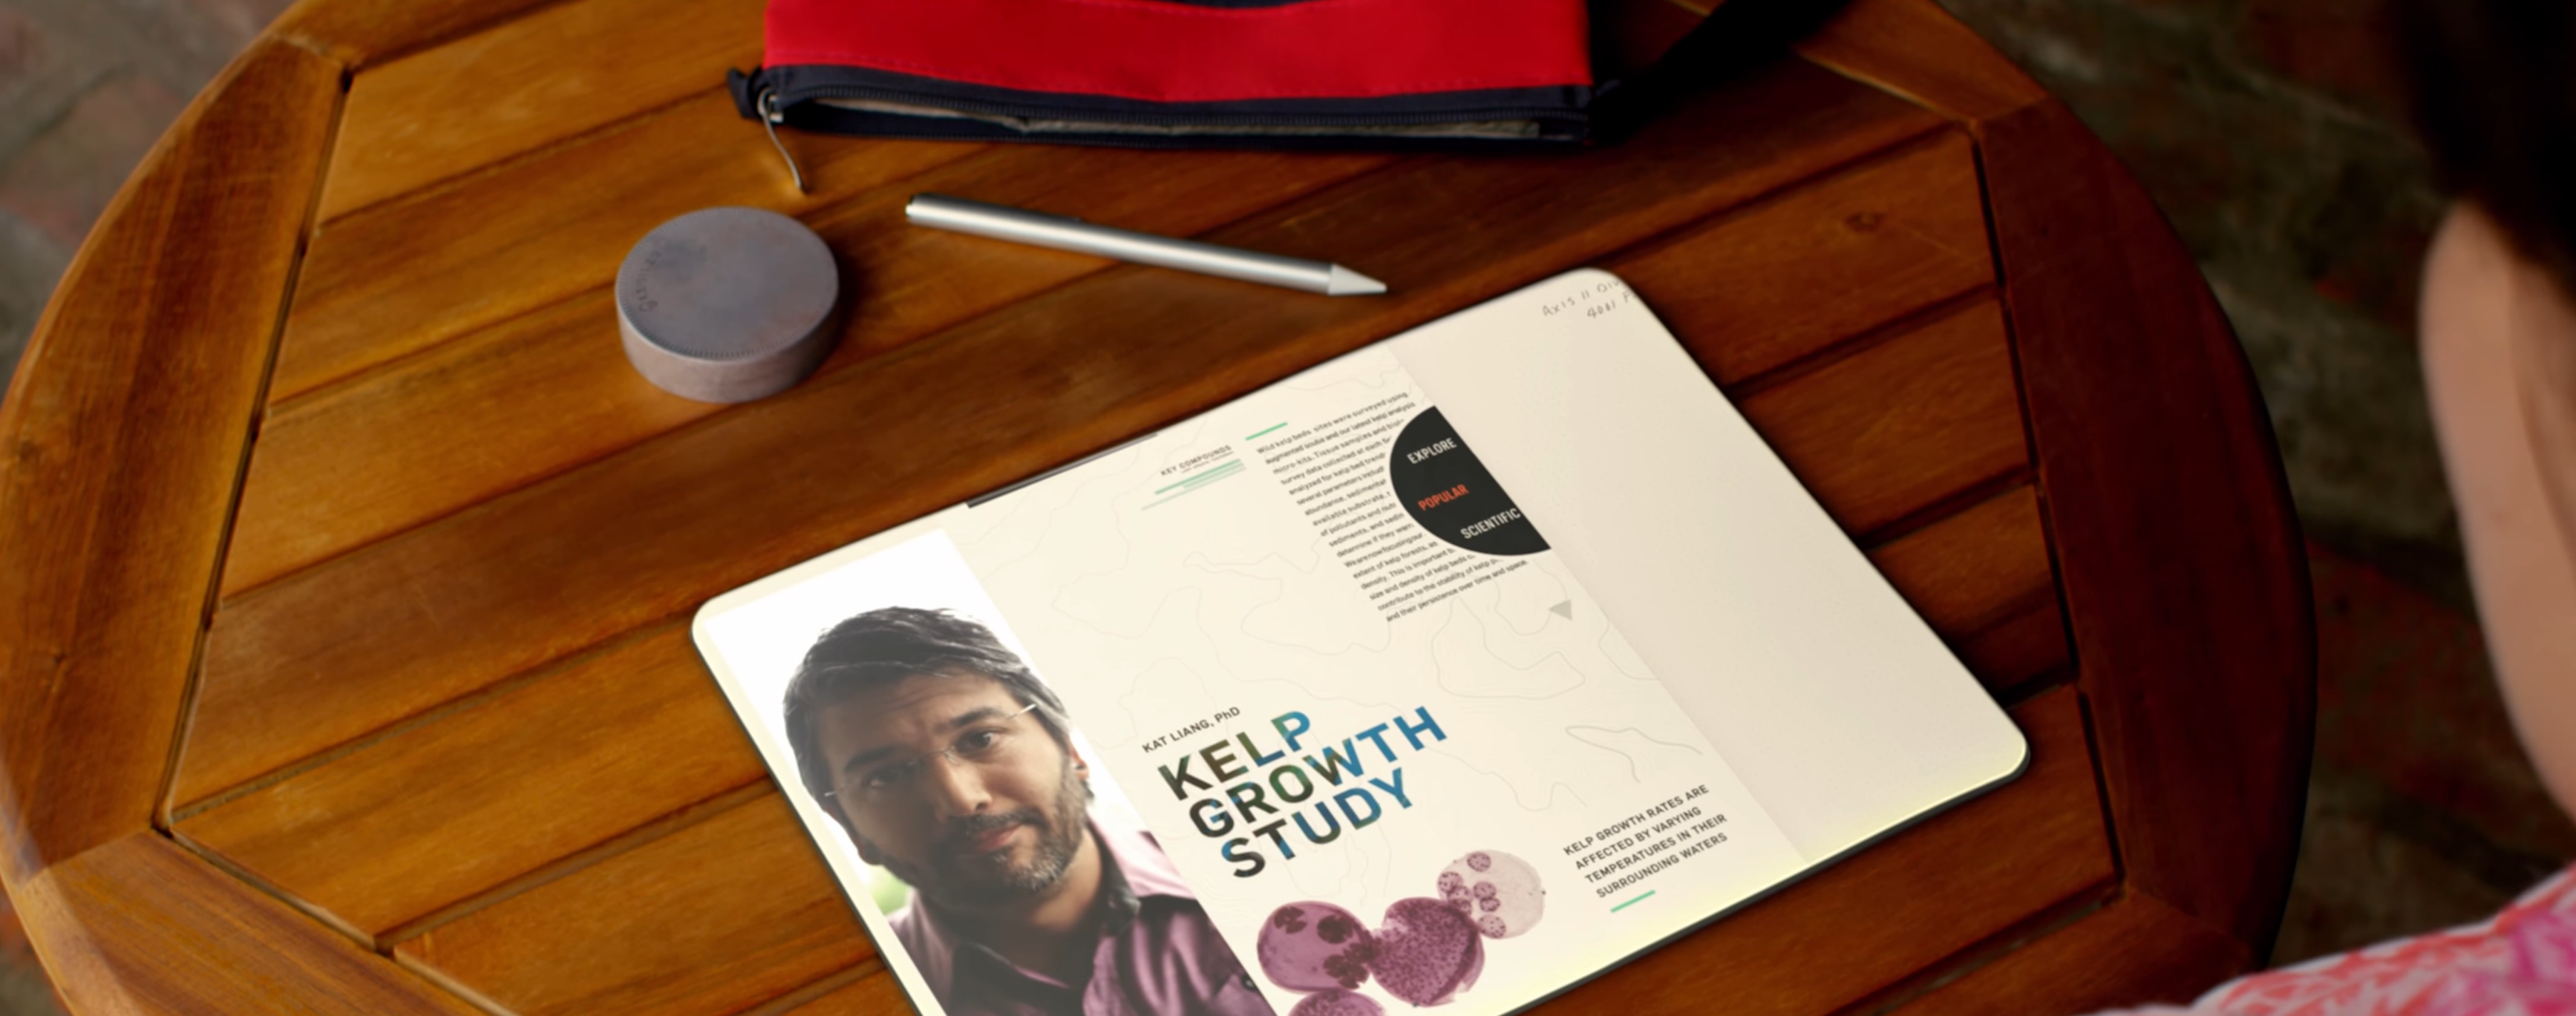
\includegraphics[width=1\textwidth]{images/ProSocialTeamwork.png}
    \caption{Snapshot of leisurely activity, demonstrating alignment towards quality education}
    \label{fig:edu}
\end{figure}  

\begin{figure}[H]
    \centering
    \includegraphics[width=1\textwidth]{images/ProFood.png}
    \caption{Snapshot of kelp farm planning, demonstrating alignment towards zero hunger}
    \label{fig:food}
\end{figure}  

\begin{figure}[H]
    \centering
    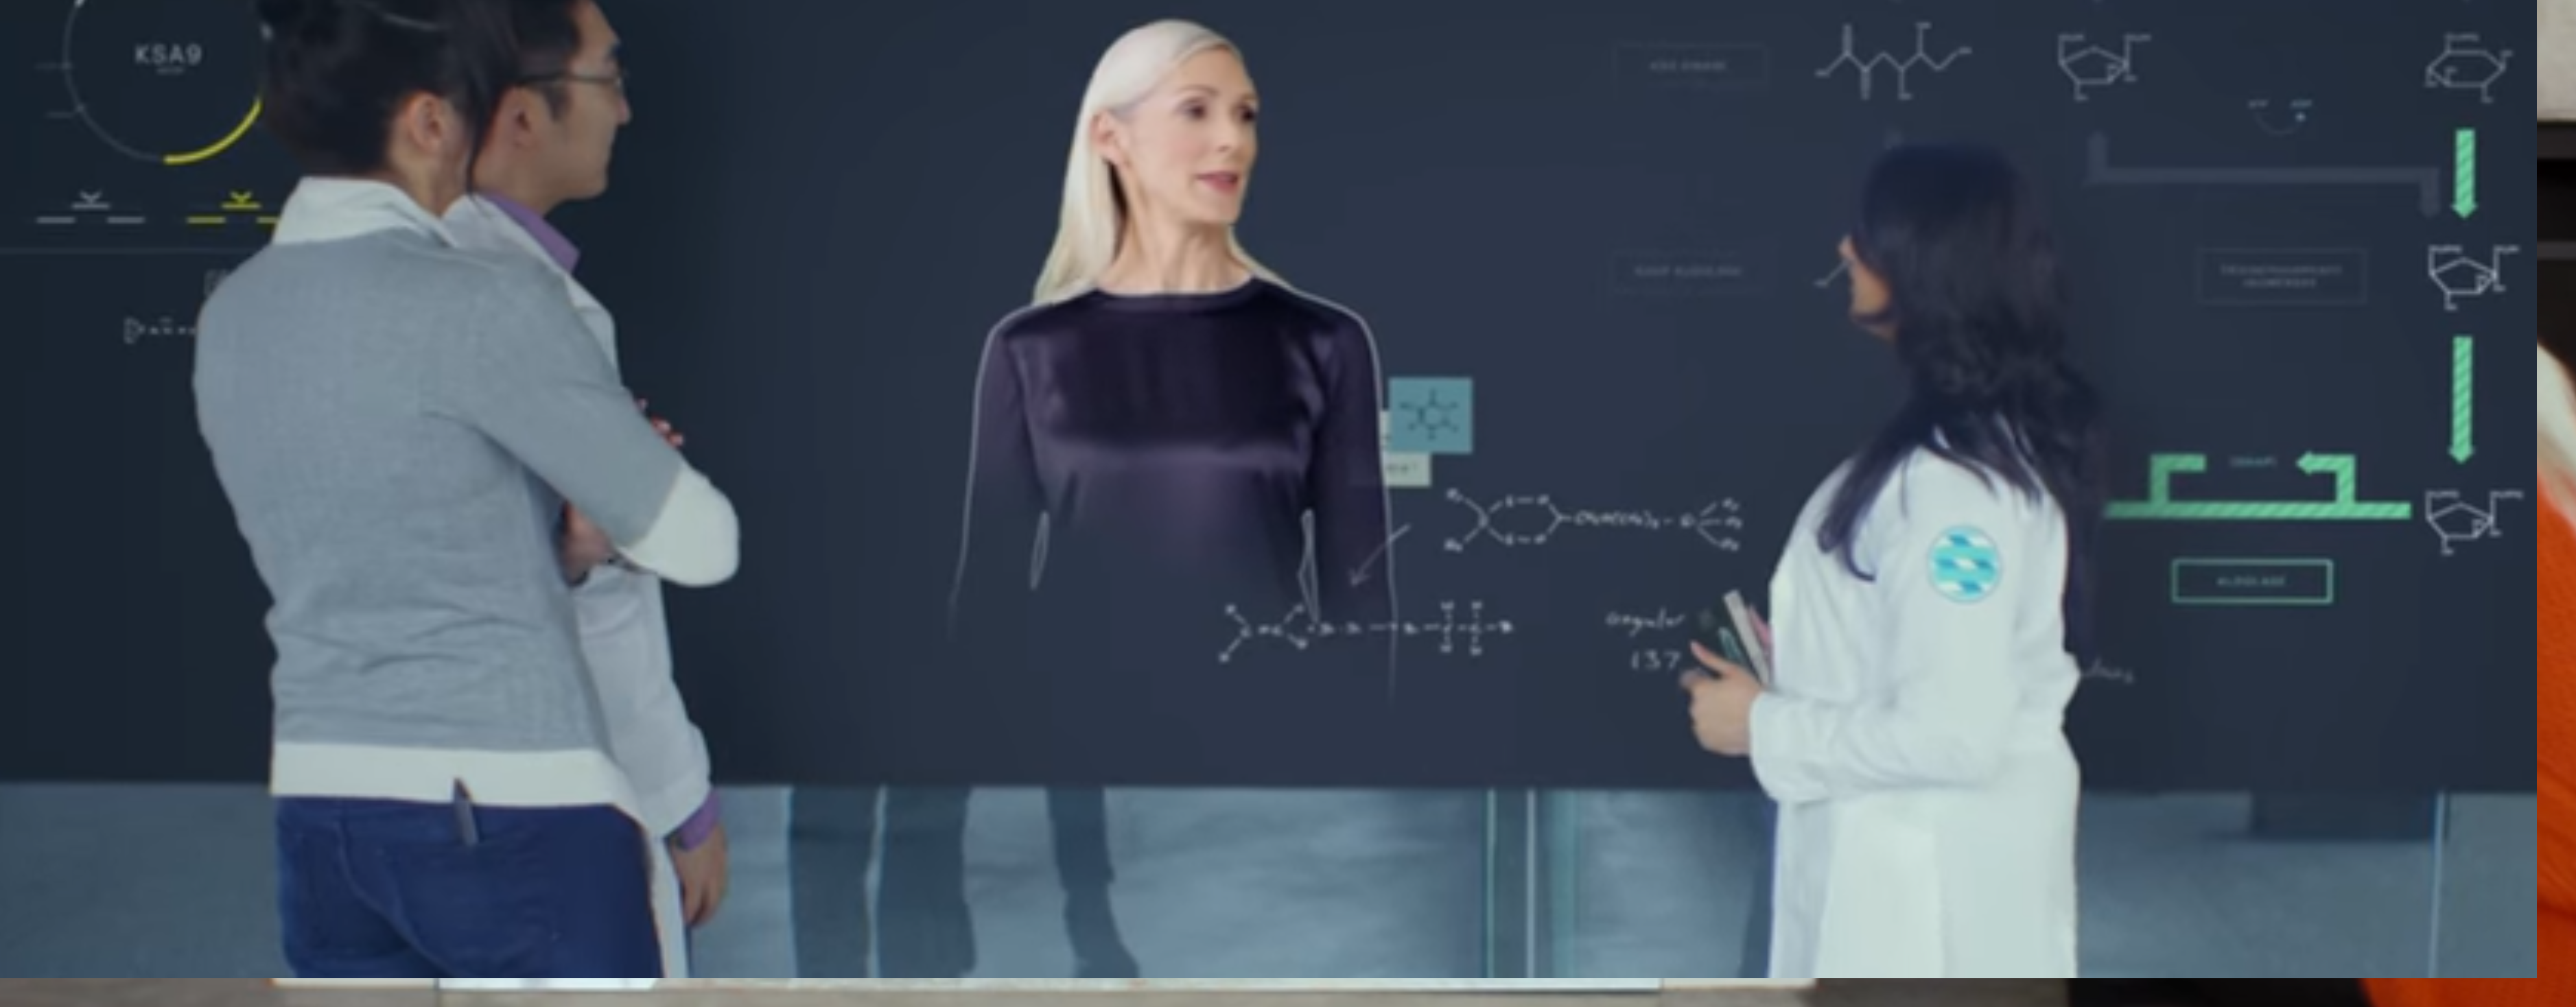
\includegraphics[width=1\textwidth]{images/ProCollab.png}
    \caption{Snapshot of active research discussion, demonstrating alignment towards international collaboration}
    \label{fig:collab}
\end{figure}  

\begin{figure}[H]
    \centering
    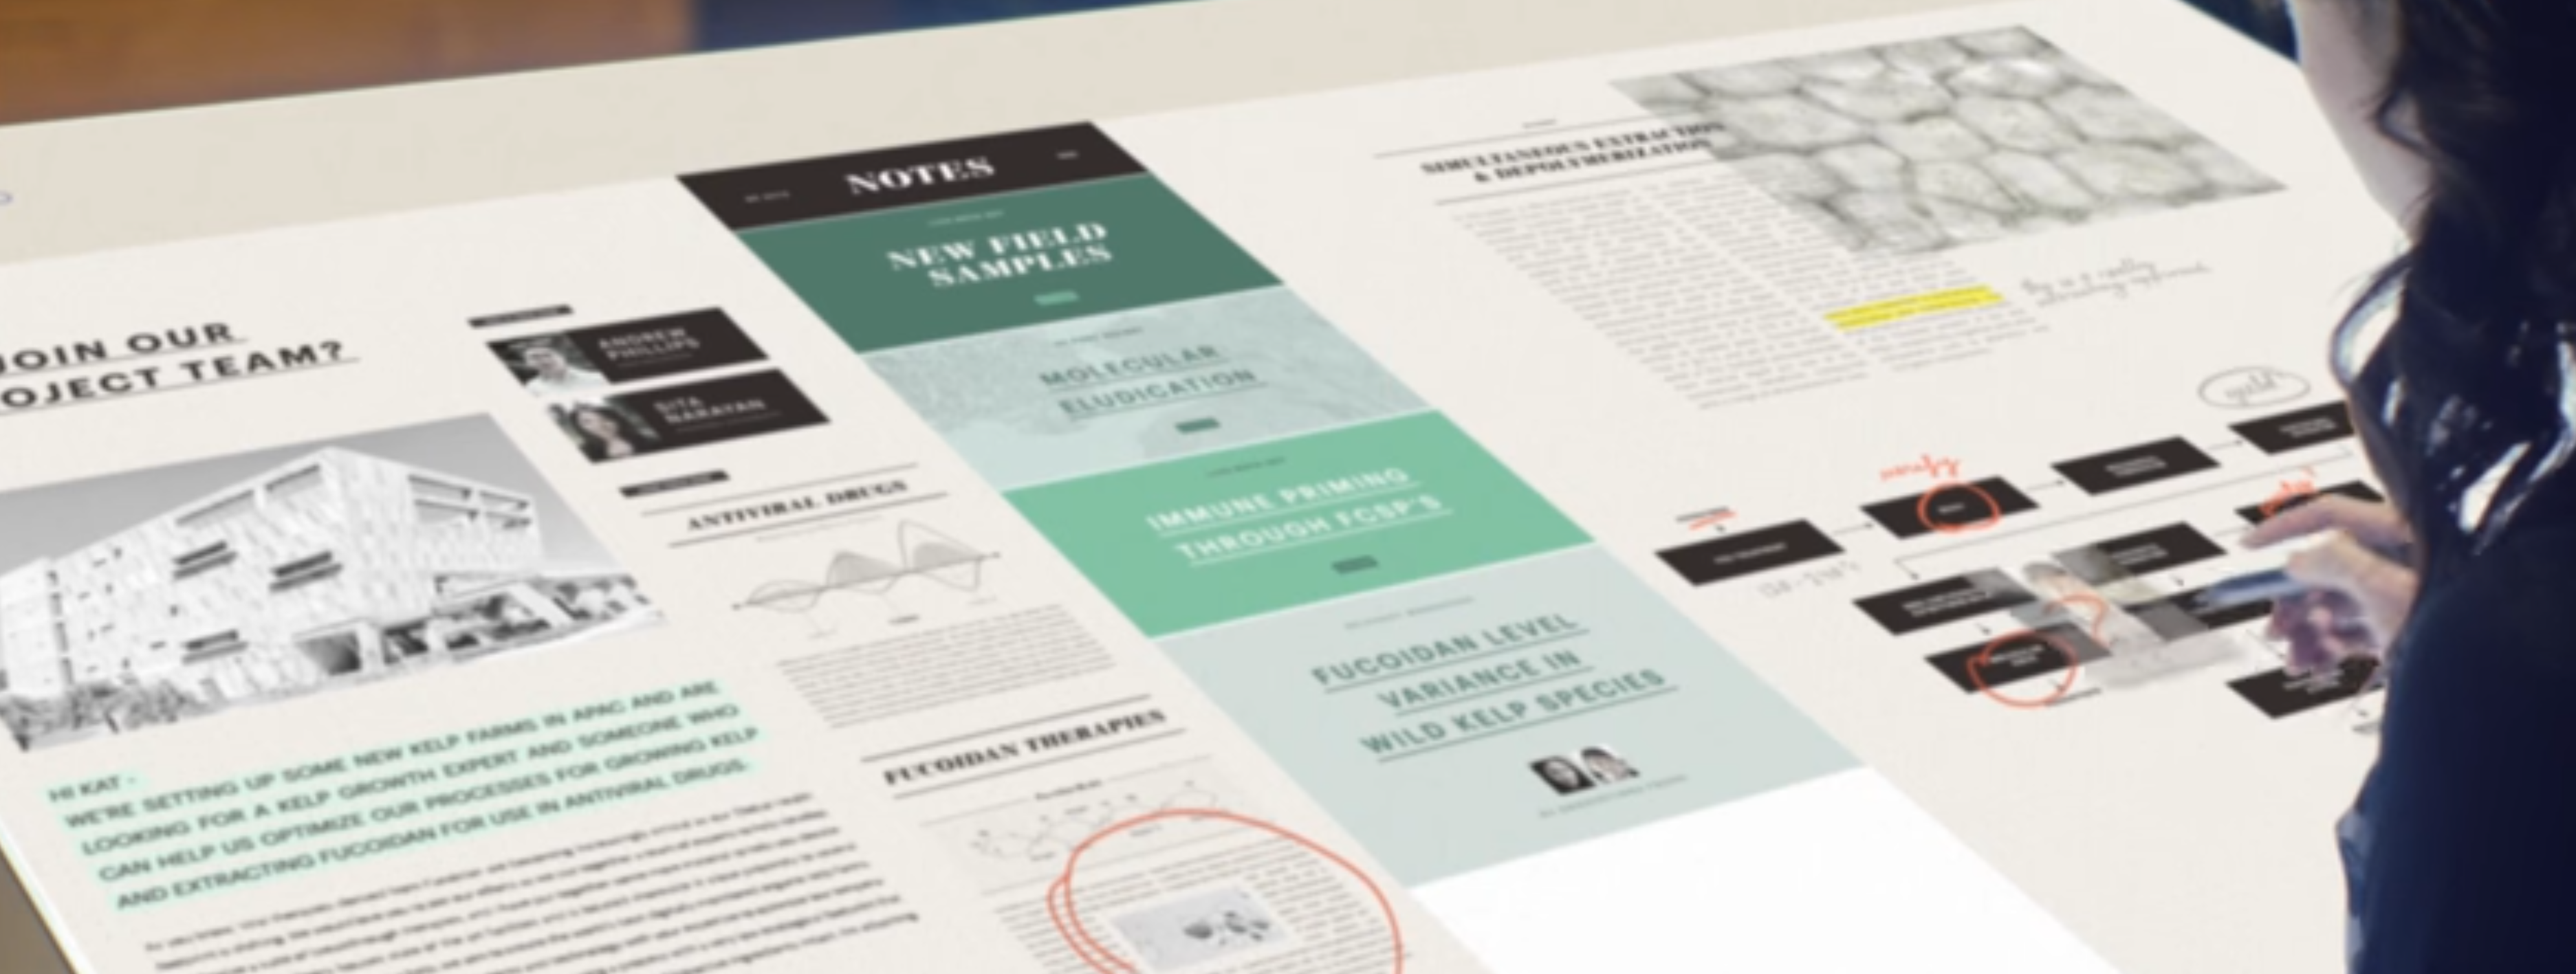
\includegraphics[width=1\textwidth]{images/ProEfficiency.png}
    \caption{Snapshot of workspace, demonstrating alignment towards efficiency}
    \label{fig:work}
\end{figure} 

\begin{figure}[H]
    \centering
    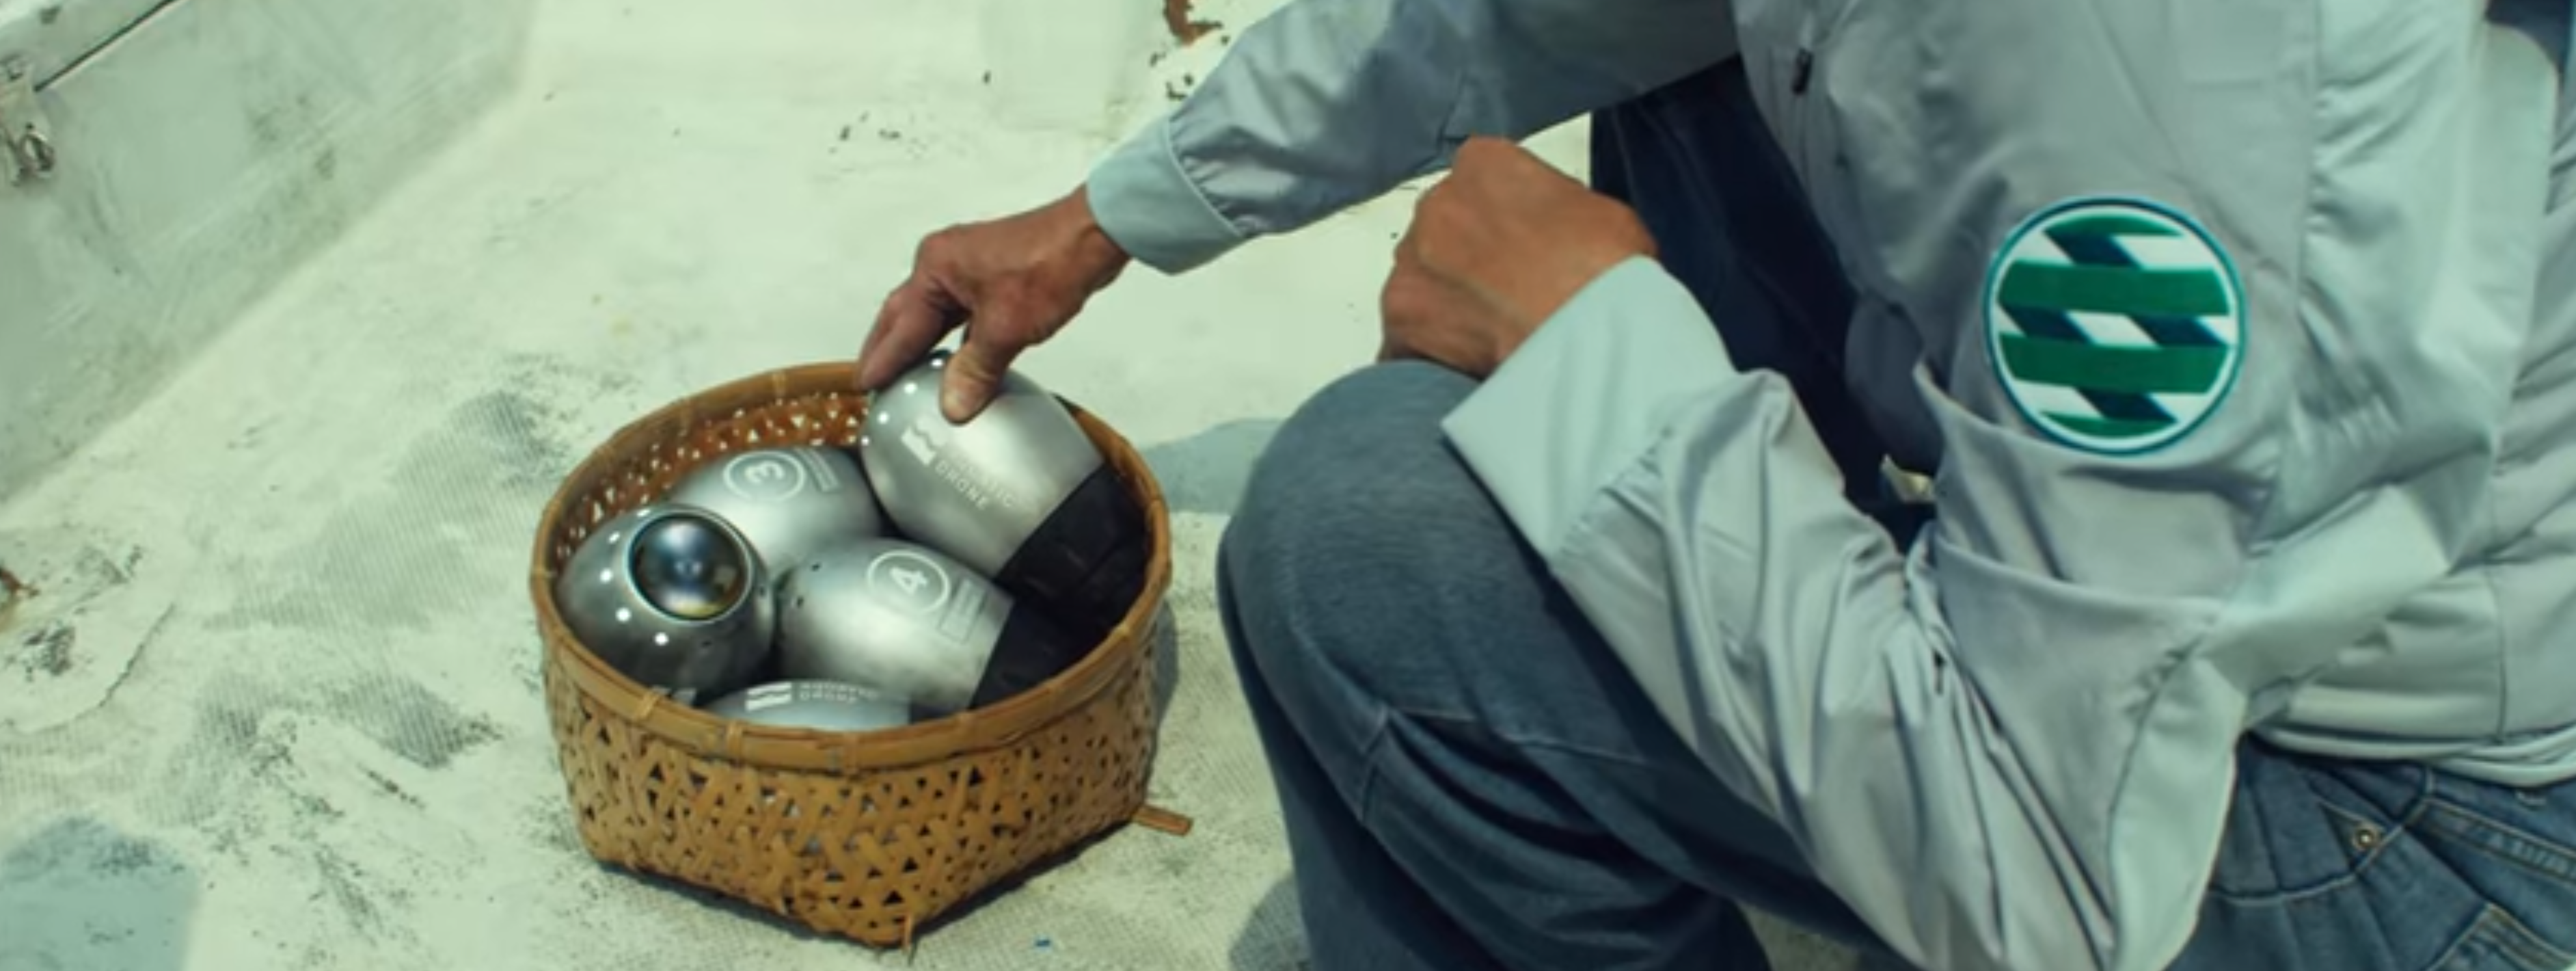
\includegraphics[width=1\textwidth]{images/ProMachines.png}
    \caption{Snapshot of machines being activated, demonstrating alignment towards machine assisted labor}
    \label{fig:labor}
\end{figure} 

\begin{figure}[H]
    \centering
    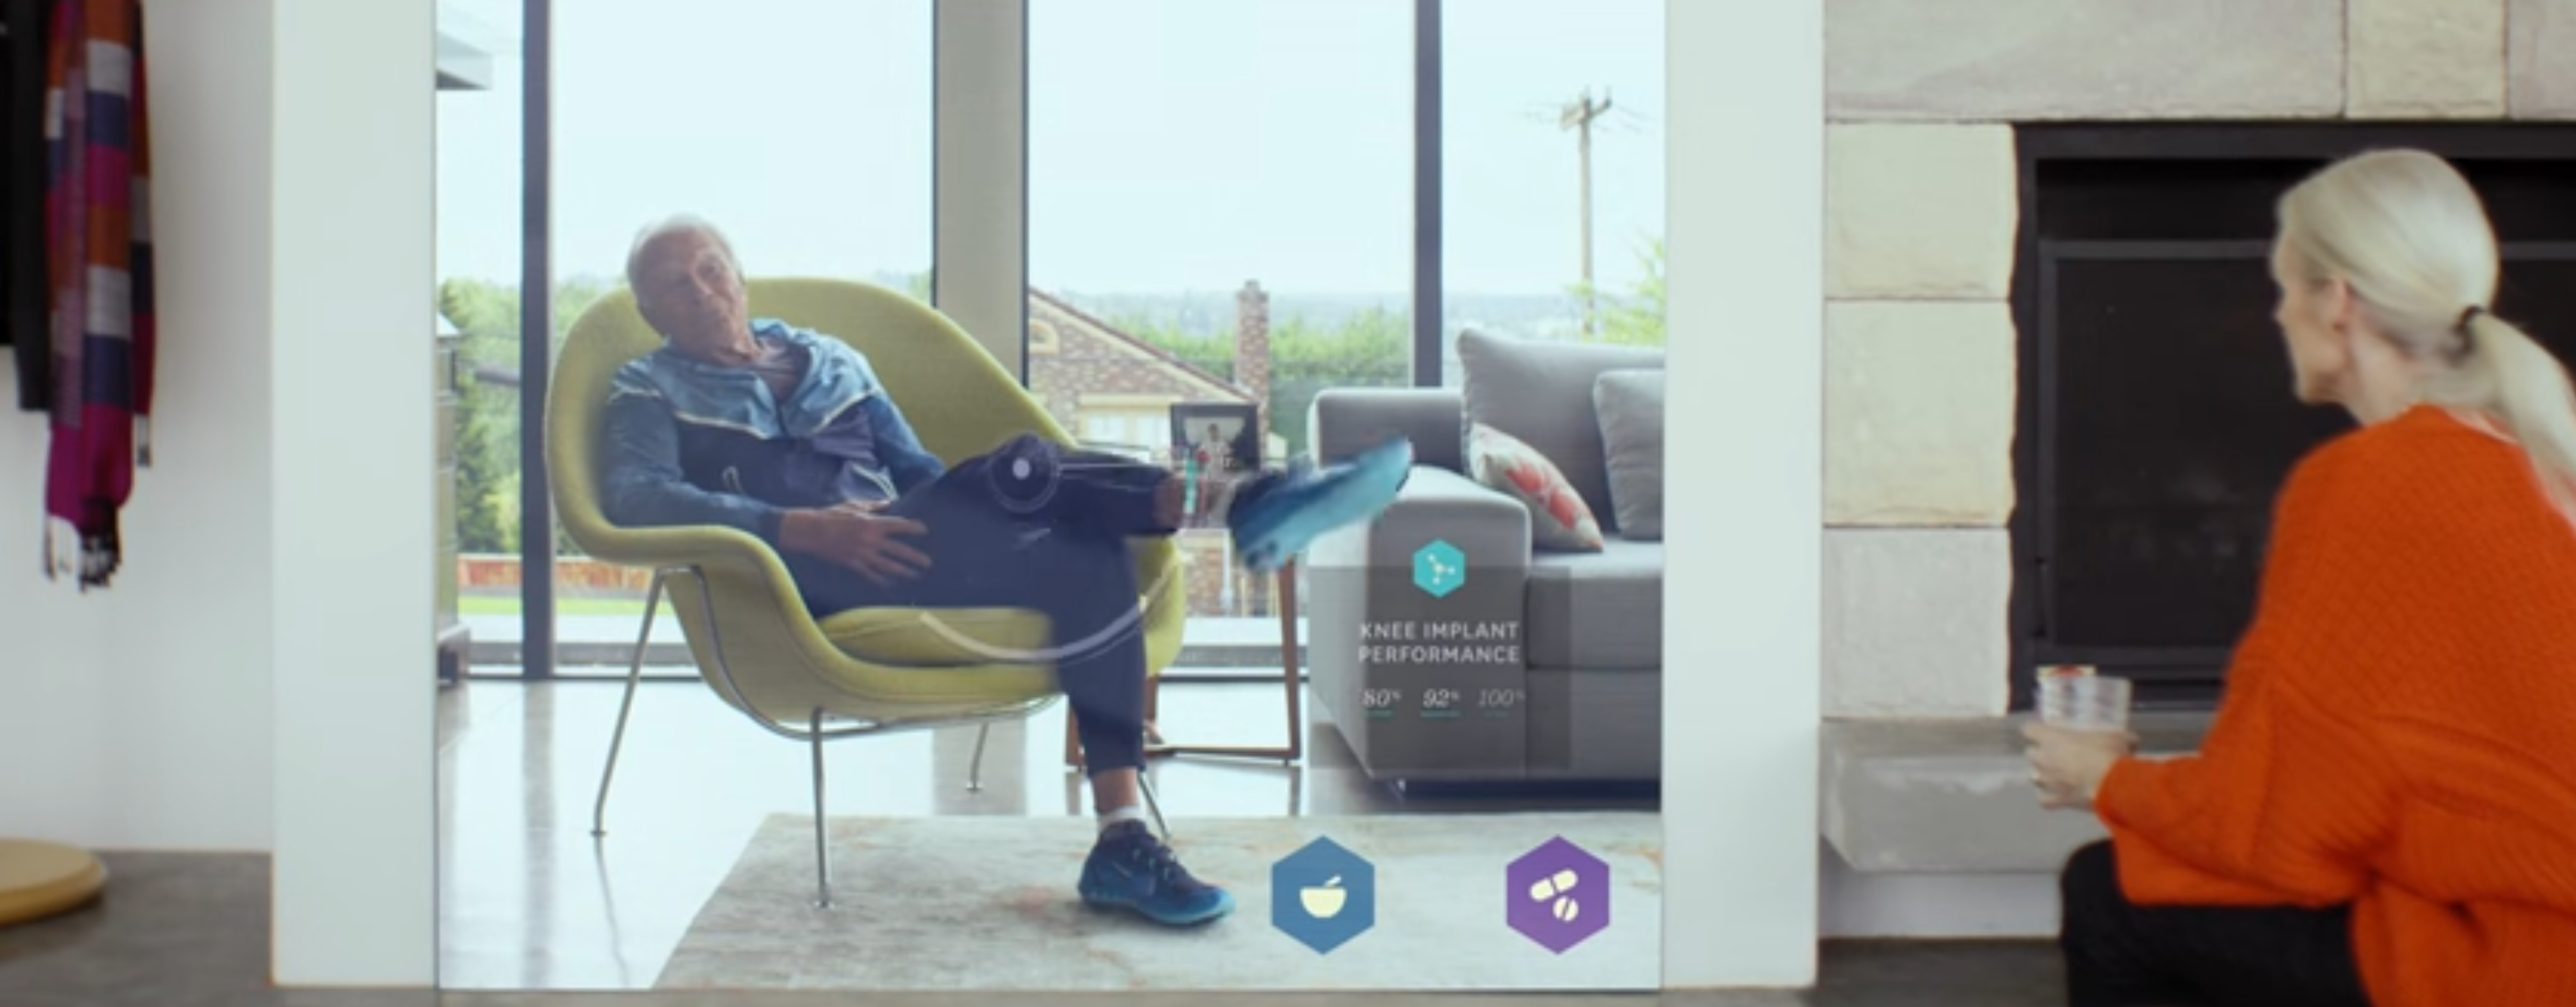
\includegraphics[width=1\textwidth]{images/ProHealthAndSocialInteraction.png}
    \caption{Snapshot of living room social interaction, demonstrating alignment towards good health and wellbeing}
    \label{fig:social}
\end{figure} 

\begin{figure}[H]
    \centering
    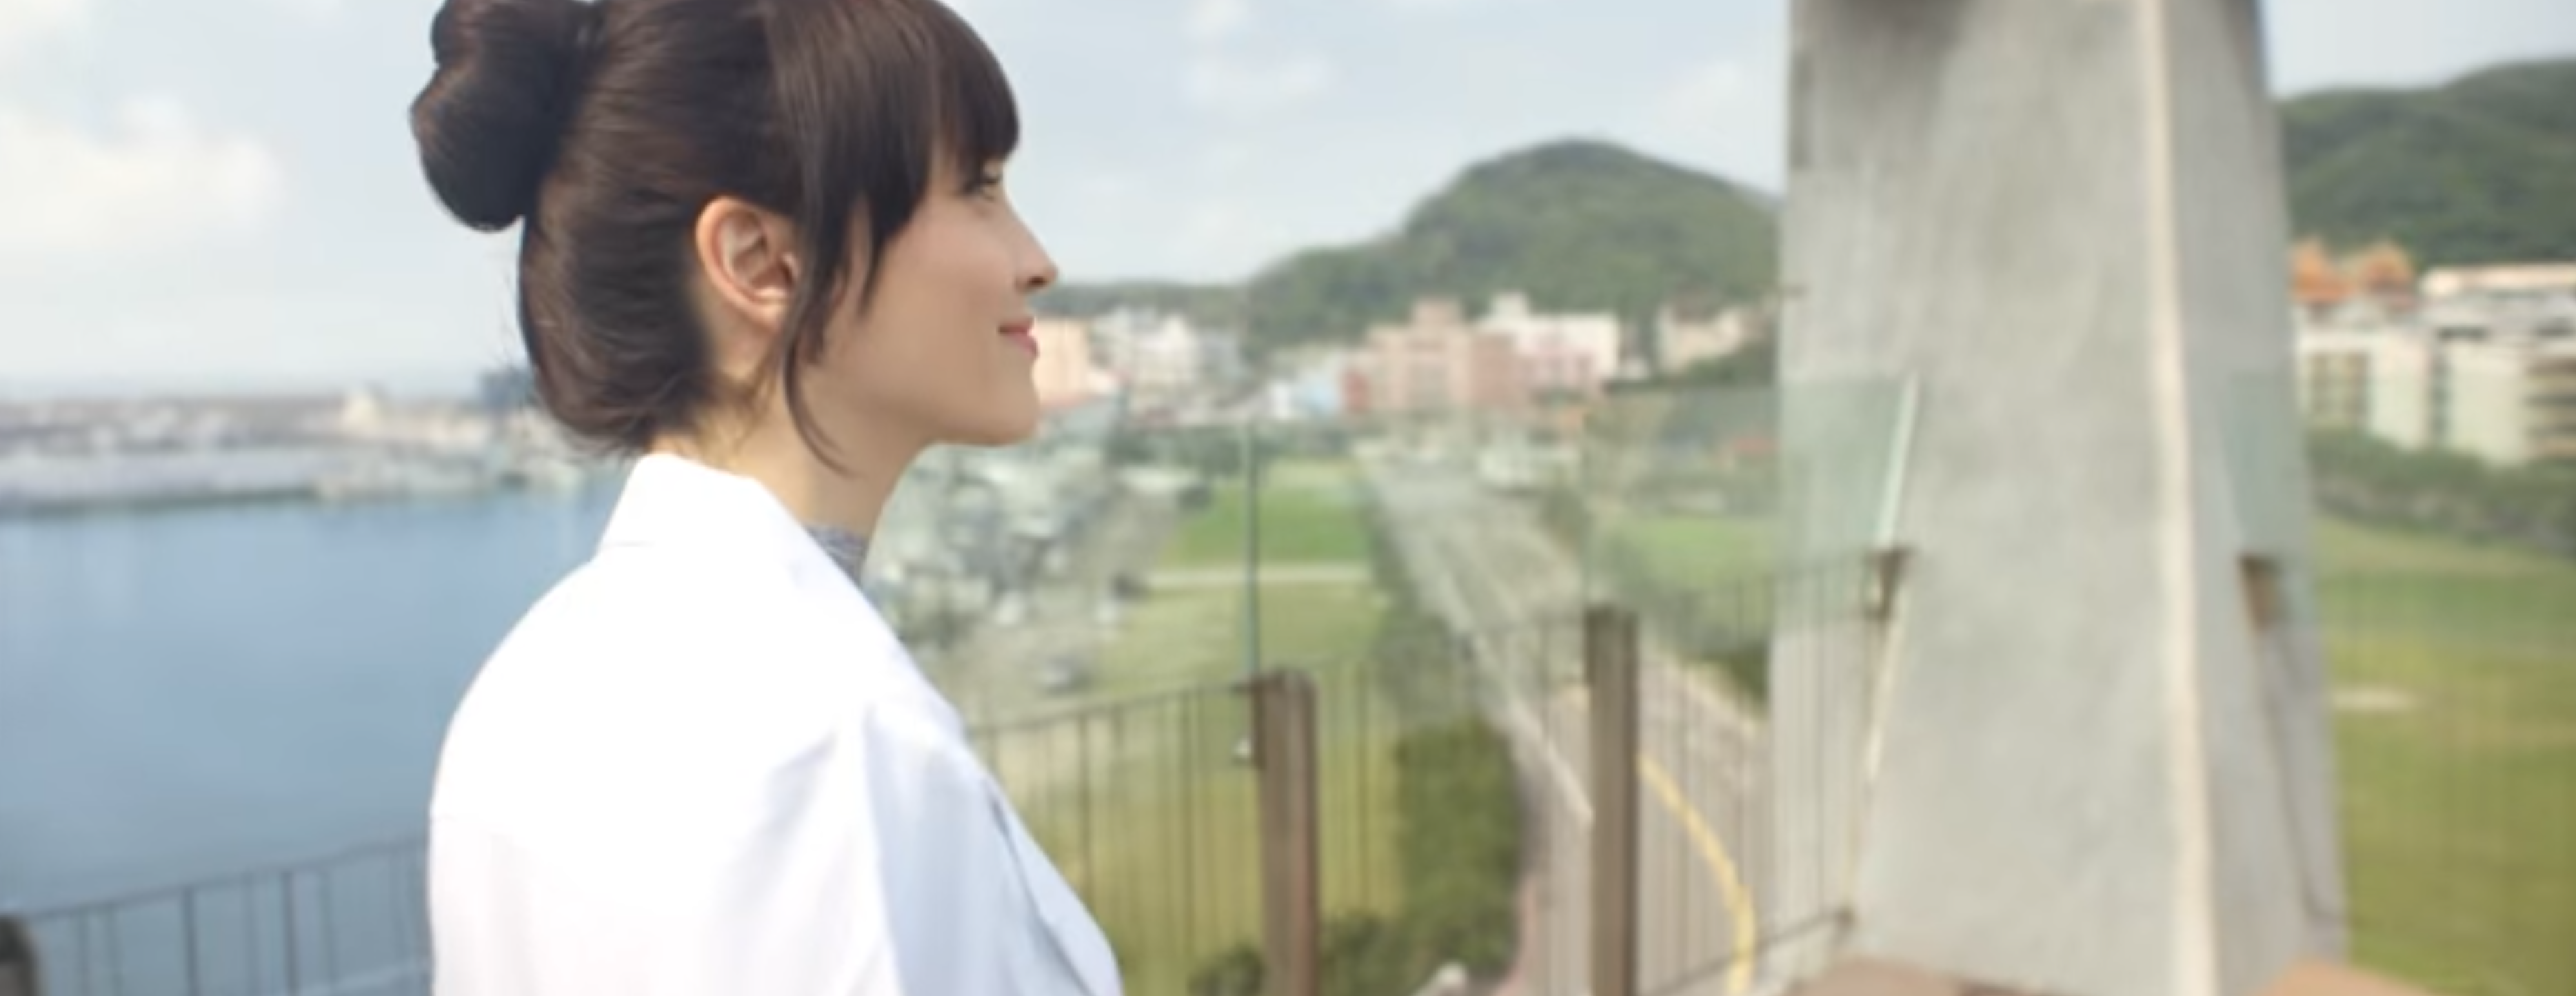
\includegraphics[width=1\textwidth]{images/ProClimate.png}
    \caption{Snapshot of women taking fresh air in a tempered climate, demonstrating alignment towards climate}
    \label{fig:fresh}
\end{figure} 

\subsubsection*{Notes}
\begin{itemize}
    \item At no point was physical activity shown, except for very mild intensity activity like walking or pouring tea.
    \item During the video, a music track best described as inciting "wonderous" feelings is playing.
    \item The video is showcasing a future of almost complete sustainability and becoming unbound from physical limitations.
\end{itemize}

\subsection{Practises}

\begin{itemize}
    \item Children will be learning through highly technological equipment, that can take them very close to the subject of discovery (figure ~\ref{fig:teach}).
    \item Research is carried out by people all around the world, with leisure time being part of the contribution towards technological progress (figure ~\ref{fig:edu},~\ref{fig:collab}).
    \item Food production is expanded to kelp farming, and only requires planning with a technological device (figure ~\ref{fig:food}).
    \item Physical activity is very limited, so much that most if not all of the physical labor is done by autonomous robots (figure ~\ref{fig:labor} ).
    \item Social interactions will no longer be limited by physical distance, and problems related to health and wellbeing are solved (figure ~\ref{fig:social} ).
    \item Humans no longer compromise the environment whether it be life on land, underwater or the climate with any actions (figure ~\ref{fig:teach},~\ref{fig:nature},~\ref{fig:fresh}).
    \item Humans are no longer bound by language barriers, as technology will be translating everything real-time (figure ~\ref{fig:teach}).
\end{itemize}

\subsection{Inteded demographic}
The future is for the well-off, ie. those with a high income, high education and high living standards that can afford high-tech solutions. 
The future is not bound by geography, race or gender. The vast majority of places shown are not geographically specific, and most if not all races and genders are represented.

\subsection{Assumptions}
Although not explicitly shown, it is assumed that energy is produced from renewable sustainable sources. 
